\documentclass{beamer}
\usetheme{CambridgeUS}
\usepackage{listings}
\usepackage{blkarray}
\usepackage{listings}
\usepackage{subcaption}
\usepackage{url}
\usepackage{tikz}
\usepackage{tkz-euclide} % loads  TikZ and tkz-base
%\usetkzobj{all}
\usetikzlibrary{calc,math}
\usepackage{float}
\renewcommand{\vec}[1]{\mathbf{#1}}
\usepackage[export]{adjustbox}
\usepackage[utf8]{inputenc}
\usepackage{amsmath}
\usepackage{amsfonts}
\usepackage{tikz}
\usepackage{hyperref}
\usepackage{bm}
\usetikzlibrary{automata, positioning}
\providecommand{\pr}[1]{\ensuremath{\Pr\left(#1\right)}}
\providecommand{\mbf}{\mathbf}
\providecommand{\qfunc}[1]{\ensuremath{Q\left(#1\right)}}
\providecommand{\sbrak}[1]{\ensuremath{{}\left[#1\right]}}
\providecommand{\lsbrak}[1]{\ensuremath{{}\left[#1\right.}}
\providecommand{\rsbrak}[1]{\ensuremath{{}\left.#1\right]}}
\providecommand{\brak}[1]{\ensuremath{\left(#1\right)}}
\providecommand{\lbrak}[1]{\ensuremath{\left(#1\right.}}
\providecommand{\rbrak}[1]{\ensuremath{\left.#1\right)}}
\providecommand{\cbrak}[1]{\ensuremath{\left\{#1\right\}}}
\providecommand{\lcbrak}[1]{\ensuremath{\left\{#1\right.}}
\providecommand{\rcbrak}[1]{\ensuremath{\left.#1\right\}}}
\providecommand{\abs}[1]{\vert#1\vert}
\newcommand*{\permcomb}[4][0mu]{{{}^{#3}\mkern#1#2_{#4}}}
\newcommand*{\perm}[1][-3mu]{\permcomb[#1]{P}}
\newcommand*{\comb}[1][-1mu]{\permcomb[#1]{C}}
\renewcommand{\thetable}{\arabic{table}} 
\newcounter{saveenumi}
\newcommand{\seti}{\setcounter{saveenumi}{\value{enumi}}}
\newcommand{\conti}{\setcounter{enumi}{\value{saveenumi}}}
\usepackage{amsmath}
\setbeamertemplate{caption}[numbered]{}
\DeclareUnicodeCharacter{2212}{\textendash}
\title{AI1110 Assignment 7}
\author{SADINENI ABHINAY-CS21BTECH11055}
\date{\today}
\logo{\large \LaTeX{}}
\begin{document}
	
	\begin{frame}
		\titlepage
	\end{frame}

\begin{frame}{Outline}
  \tableofcontents
\end{frame}

\section{Abstract}
	\begin{frame}{Abstract}
		\begin{itemize}
			\item 	This document contains the solution to Question of Chapter 13 (Probability) in the NCERT Class 12 Textbook.
		\end{itemize}
	\end{frame}
	
	\section{Question}
	\begin{frame}{Question}
		\begin{block}{\textbf{Probability  ex 13.5 q8.}}
			 Suppose X has a binomial distribution $B\brak{6,\frac{1}{2}}$ .Show that $X=3$ is most likely outcome.
			 \brak{hint: \pr{X=3} \text{is the max among all} \pr{x_i}, x_{i}=0,1,2,3,4,5,6}
		\end{block}
	\end{frame}
	

	\section{Theory}
	\begin{frame}{Theory}
			 \begin{block}{Binomial Distribution}
	      the binomial distribution with parameters n and p is the discrete probability distribution of the number of successes in a sequence of n independent experiments, each asking a yes–no question, and each with its own Boolean-valued outcome: success (with probability p) or failure (with probability $q = 1 − p$)
		\end{block}	   
			      The Expression is given by:
\begin{align}
\sum_{i=0}^{n}\pr{X = i} =  \sum_{i=0}^{n} \comb{n}{i}(\text{p})^i\left(1-\text{p}\right)^{n-i}
\\
\pr{X = i} =\comb{n}{i}(\text{p})^i\left(1-\text{p}\right)^{n-i}
	      \end{align}
	\end{frame}
	\section{Solution}	
	\begin{frame}{Solution}
		Given X has binomial distribution B\brak{6,\frac{1}{2}} ,Now let us find out individiual probabilities for all $i=0,1,2,3,4,5,6$,here $n=6$ and $p=\frac{1}{2}$.
		\begin{align}
		\pr{X = 0} &=\comb{6}{0}(\frac{1}{2})^0\left(\frac{1}{2}\right)^{6-0}=\frac{1}{64} \\
			\pr{X = 1}& =\comb{6}{1}(\frac{1}{2})^6=\frac{3}{32}\\
			\pr{X = 2} &=\comb{6}{2}(\frac{1}{2})^6=\frac{15}{64}\\
			\pr{X = 3} &=\comb{6}{3}(\frac{1}{2})^6=\frac{5}{16}
		\end{align}
	\end{frame}

	\begin{frame}{}
	\begin{align}
	\pr{X = 4} &=\comb{6}{4}(\frac{1}{2})^6=\frac{15}{64}\\
			\pr{X = 5} &=\comb{6}{5}(\frac{1}{2})^6=\frac{3}{32}\\
			\pr{X = 6} &=\comb{6}{6}(\frac{1}{2})^6=\frac{1}{64}
	\end{align}
		\begin{table}[ht!]
	\centering
	 {
	\begin{tabular}{|c|c|}
		\hline
		\textbf{Probability}&\textbf{Value}\\
		\hline
		$\pr{X=0}$ &0.016 \\
		\hline
	$\pr{X=1}$ &0.094 \\
		\hline
	$\pr{X=2}$ &0.234 \\
		\hline
	$\pr{X=3}$ &0.312 \\
		\hline
	$\pr{X=4}$ &0.234 \\
	       \hline
	$\pr{X=5}$ &0.094 \\
	       \hline
	$\pr{X=6}$ &0.016 \\
	       \hline
	\end{tabular}
}

	\caption{Values}
	\label{table:1}
    \end{table}
	\end{frame}

\begin{frame}{}
From the Table-1 we come to know that $\pr{X=3}$ has the maximum among all the values ,We can also verify from the PMF plot in following section, at $X=3$ it has the highest y-value\brak{\text{probability},\pr{X=i}}
$\therefore X=3$ is most likely outcome.

\end{frame}
\section{PMF}
\begin{frame}{PMF}
\begin{figure}[!ht]
		\centering
			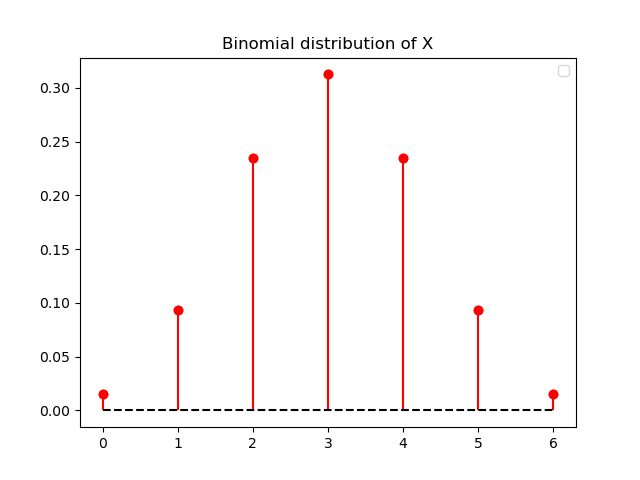
\includegraphics[width=\textwidth,height=5.5cm,keepaspectratio]{figs/binomial1.png}
		\caption{PMF}
		\label{Fig 0:}
	\end{figure}
\end{frame}
\end{document}
